\documentclass[tikz,border=10pt]{standalone}
\usepackage{tikz}
\usetikzlibrary{arrows.meta,positioning,shapes}
\usepackage{amsmath} % <<<<<<  AÑADIDO


\begin{document}

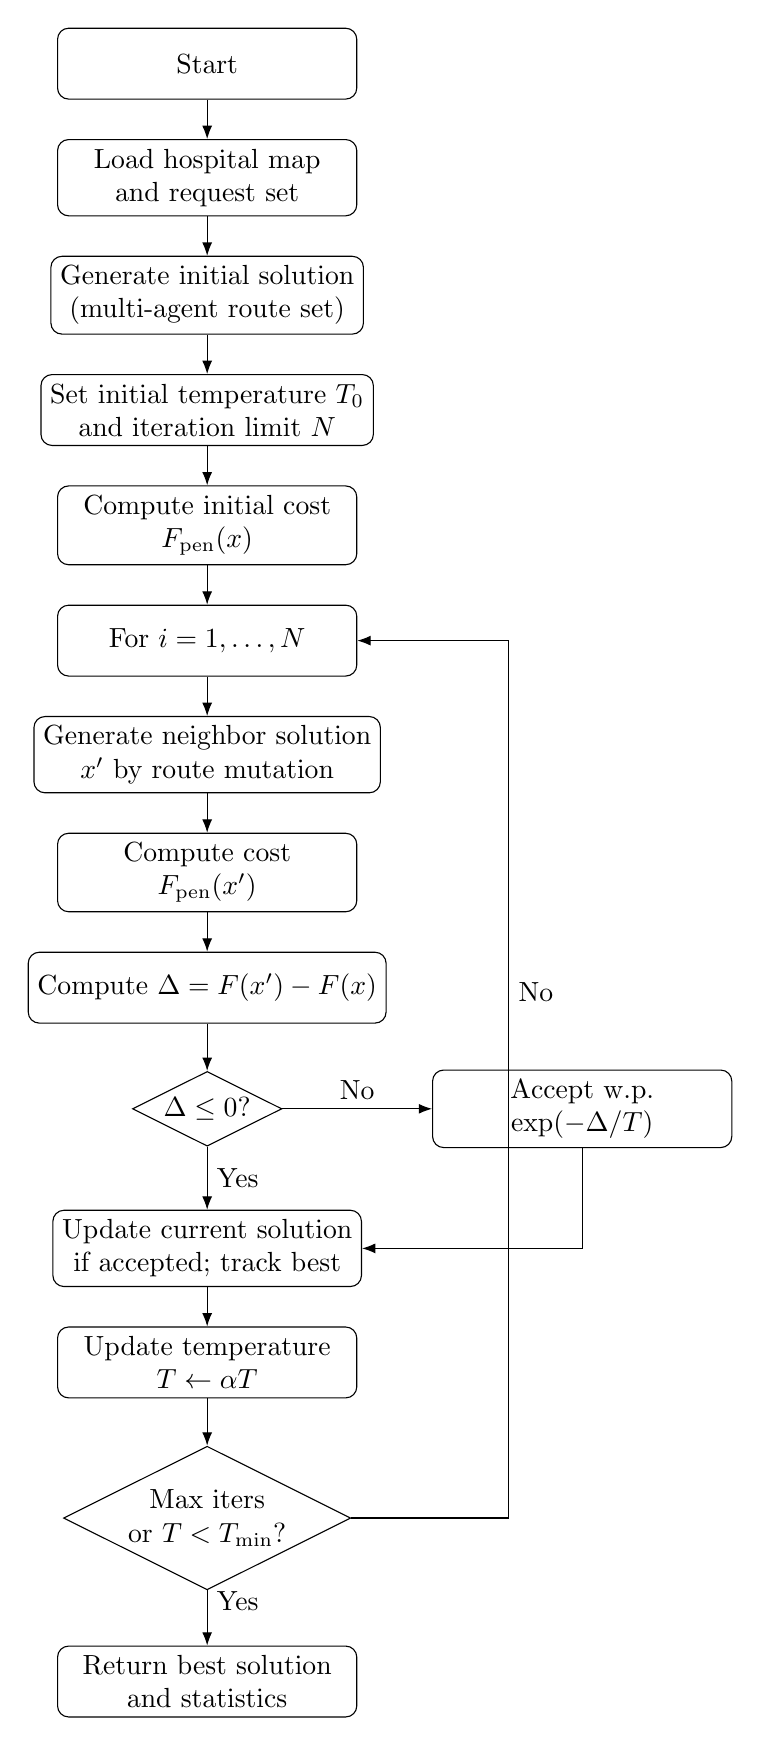
\begin{tikzpicture}[
  node distance=0.5cm,
  >=Latex,
  block/.style={rectangle, draw, rounded corners, align=center, minimum width=3.8cm, minimum height=0.9cm},
  decision/.style={diamond, draw, aspect=2, align=center, inner sep=1pt},
  line/.style={draw, -{Latex}}
]

\node[block] (start) {Start};
\node[block, below=of start] (env) {Load hospital map\\and request set};
\node[block, below=of env] (init) {Generate initial solution\\(multi-agent route set)};
\node[block, below=of init] (setT) {Set initial temperature $T_0$\\and iteration limit $N$};
\node[block, below=of setT] (eval0) {Compute initial cost\\$F_{\text{pen}}(x)$};
\node[block, below=of eval0] (loop) {For $i=1,\dots,N$};
\node[block, below=of loop] (neighbor) {Generate neighbor solution\\$x'$ by route mutation};
\node[block, below=of neighbor] (evaln) {Compute cost\\$F_{\text{pen}}(x')$};
\node[block, below=of evaln] (delta) {Compute $\Delta = F(x')-F(x)$};
\node[decision, below=of delta, yshift=-0.1cm] (accept) {$\Delta \le 0$?};
\node[block, right=1.9cm of accept] (metropolis) {Accept w.p.\\$\exp(-\Delta/T)$};
\node[block, below=of accept, yshift=-0.3cm] (updatex) {Update current solution\\if accepted; track best};
\node[block, below=of updatex] (cool) {Update temperature\\$T \leftarrow \alpha T$};
\node[decision, below=of cool, yshift=-0.1cm] (stop) {Max iters\\or $T<T_{\min}$?};
\node[block, below=of stop, yshift=-0.2cm] (end) {Return best solution\\and statistics};

\path[line] (start) -- (env);
\path[line] (env) -- (init);
\path[line] (init) -- (setT);
\path[line] (setT) -- (eval0);
\path[line] (eval0) -- (loop);
\path[line] (loop) -- (neighbor);
\path[line] (neighbor) -- (evaln);
\path[line] (evaln) -- (delta);
\path[line] (delta) -- (accept);

\path[line] (accept.east) -- node[above]{No} (metropolis.west);
\path[line] (metropolis.south) |- (updatex.east);
\path[line] (accept.south) -- node[right]{Yes} (updatex.north);

\path[line] (updatex) -- (cool);
\path[line] (cool) -- (stop);

\path[line] (stop.east) -- ++(2,0) |- (loop.east) node[pos=0.3, right]{No};
\path[line] (stop.south) -- (end.north) node[pos=0.2, right]{Yes};

\end{tikzpicture}


\end{document}
